\subsection{First Experience}

\subsubsection{Simple UDP capture}

After setting Wireshark's filter to display UDP only, and visiting
\textit{www.utec.edu.pe}, the total UDP packet count was approximately 69. Most
of them were outgoing packets. Their protocols varied between DNS, MDNS, DHCP,
and QUIC.\@

\begin{figure}[htbp]
    \centering
    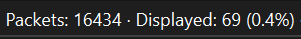
\includegraphics[width=1\linewidth]{img/1.png}
    \caption{Received UDP packet count}\label{fig:1}
\end{figure}

\begin{figure}[htbp]
    \centering
    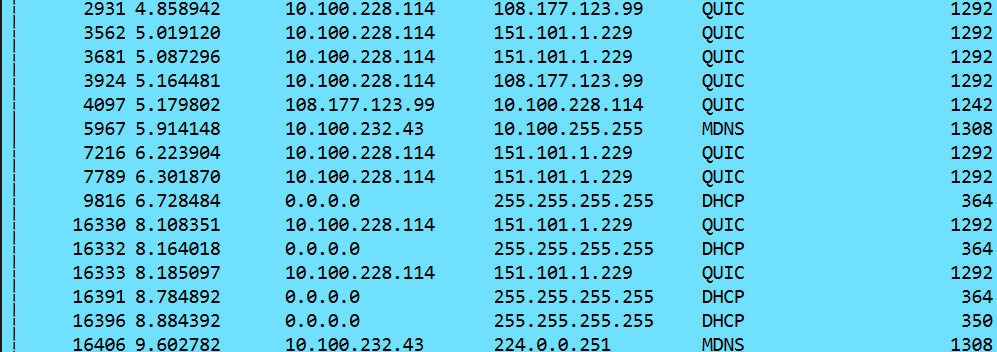
\includegraphics[width=1\linewidth]{img/2.png}
    \caption{UDP packet protocols}\label{fig:2}
\end{figure}

There were also many packets that were not necessarily related to the URL we
visited, such as a DNS query to \textit{watson.events.data.microsoft.com}. This
specific hostname is related to Windows telemetry.

\begin{figure}[htbp]
    \centering
    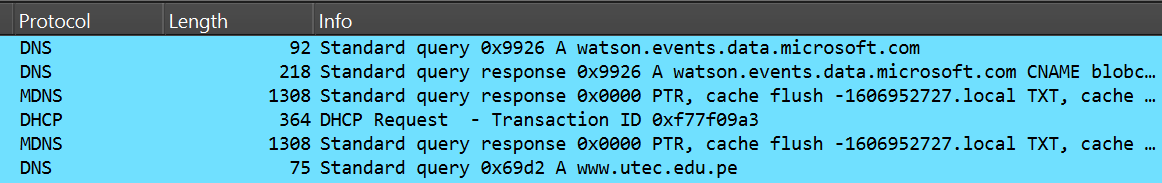
\includegraphics[width=1\linewidth]{img/3.png}
    \caption{Windows telemetry~\ensuremath{:(}}\label{fig:3}
\end{figure}

After that, we selected the first outgoing DNS packet going to
\textit{www.utec.edu.pe} to analyze its contents, which are displayed below.

\begin{figure}[htbp]
    \centering
    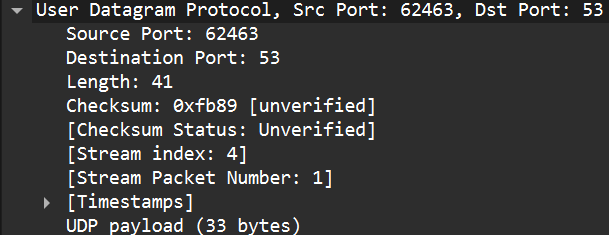
\includegraphics[width=1\linewidth]{img/4.png}
    \caption{www.utec.edu.pe packet info}\label{fig:4}
\end{figure}

The packet's main fields are:

\begin{itemize}
    \item Source/Destination Port: Port used for outgoing packet, destination port is the
          default DNS port (53).
    \item Length: Total length of the UDP packet (41 bytes).
    \item Checksum: Value used to verify the integrity of the packet.
    \item Checksum Status: Indicates whether the checksum is correct or not.
\end{itemize}

The checksum status shown in the packet is ``Unverified'', which means that the
packet's correctness was not checked. This either means that Windows 11 is not
checking the integrity of outgoing and incoming packets, or that Wireshark is
not able to verify it (most likely).

After looking around in Wireshark settings, we found a way to enable checksum
validation for UDP packets. Enabling it updated the packet info field:

\begin{figure}[htbp]
    \centering
    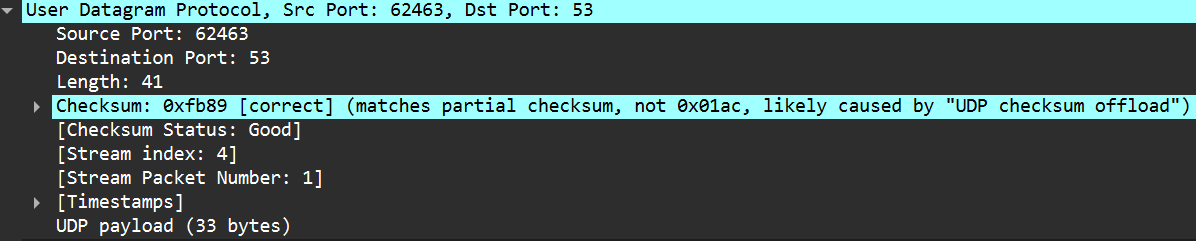
\includegraphics[width=1\linewidth]{img/5.png}
    \caption{Wireshark checksum validation}\label{fig:5}
\end{figure}

The checksum status is now ``Correct'', although it displays a message saying
that it matches the partial checksum, and that it's probably due to ``UDP
checksum offload''. A little research on this shows that it's a feature
integrated into modern NICs (Network Interface Cards) that allows them verify
the checksum, instead of having the CPU do it. This improves performance, but
it can cause small mismatches, like we saw in Wireshark.

Comparing the UDP packet info with a TCP packet, we can immediately see some
differences. There are stream indexes, TCP segments information, and most
importantly, \textbf{acknoledgment} related fields. This shows one of TCP's
particular features, handshakes.

Handshakes are a way for TCP to ensure that both servers are able to
communicate without issues. Server A sends a handshake packet to server B,
which server B then responds to with another handshake and an acknoledgment.
Finally, when server A receives it, it sends a final handshake and information
transfer can begin.

\begin{figure}[htbp]
    \centering
    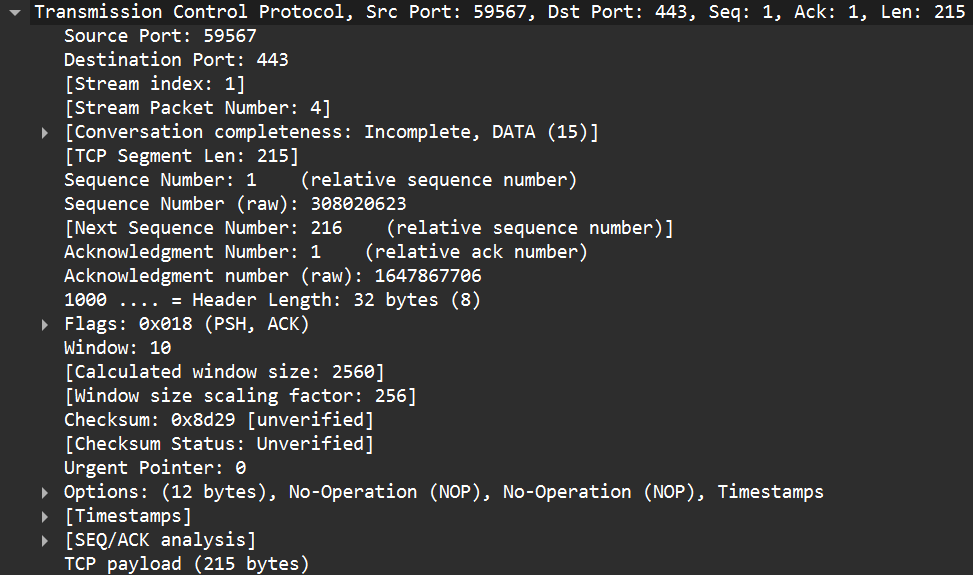
\includegraphics[width=1\linewidth]{img/6.png}
    \caption{TCP info}\label{fig:6}
\end{figure}

\subsubsection{Using nslookup}

